\chapter{Planeaci\'on}
\section{Planeaci\'on Organizacional}
\subsection{Misi\'on}
Trabajamos duro en familia para crear productos especiales e innovadores, comprometidos en acompa\~nar momentos \'unicos, generando valor para todos los integrantes.%
%
\subsection{Visi\'on}
Ser reconocidos como una panader\'ia pasteler\'ia innovadora, especial y \'unica, en b\'usqueda de lo mejor.%
%
\subsection{Valores}
\begin{itemize}
\item \emph{Honestidad}: Somos coherentes entre lo que decimos y lo que hacemos.%
\item \emph{Familiaridad}: Hornitos, dulce hogar.%
\item \emph{Compromiso}: Somos responsables de nuestros actos.%
\item \emph{Trabajo Duro}: Damos siempre la milla extra.%
\item \emph{Calidad}: Hacemos las cosas bien desde la primera vez.%
\end{itemize}
%
\section{Plan estr\'ategico de ventas}
\begin{figure}[htbp]
%centering es para centrar la imagen
	\centering
%aca es donde se incluye la imagen, se da el ancho(width), \textwidth significa que con repescto al tamano del
%texto y luego la ruta, relativa siempre es decir, a partir de donde se esta, como images esta ahi
%dentro, solo se usa desde images y ojala nada de espacios en el nombre de la imagen
		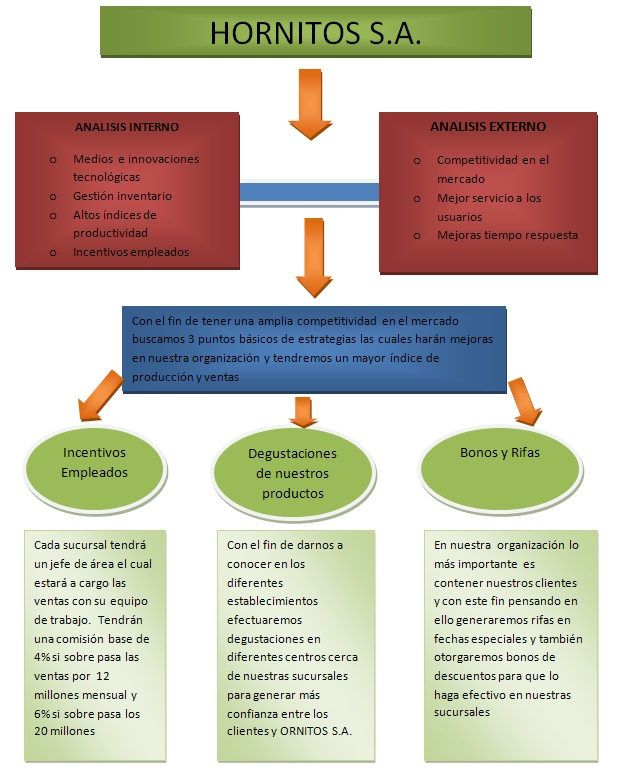
\includegraphics[width=0.60\textwidth]{images/Dibujo.jpg}
%el caption es para el texto que aparece debajo de la imagen
	\caption{Plan estrategico}
%label es para darle una referencia, por ejemplo si uno dice "como se puede ver en la imagen a1"
	\label{fig:Plan estrategico}
\end{figure}%
Hornitos S.A. Ha desarrollado una campa\~na la cual se dividir\'a en 3 partes las cuales buscara tener  por medio de los clientes una preferencia en nuestros productos e incentivar a nuestros trabajadores a tener mayor entrega con la organizaci\'on estar\'iamos hablando de tres proyectos los cuales buscaran un mejor \'ambito para la organizaci\'on.%
\\%
	\begin{itemize}
		\item Incentivos empleados.
		\item Degustaciones.
		\item bonos y rifas.
	\end{itemize}
\subsection{Incentivos empleados:}Cada sucursal tendr\'a un jefe de \'area el cual estar\'a a cargo las ventas con su  respectivo equipo de trabajo.  Tendr\'an una comisi\'on base de ventas pero con un incentivo adicional para los trabajadores y el jefe de la sucursal si logra sobre pasar ventas mensuales a 12 millones.%
\subsection{Degustaciones:} Con el fin de promocionar nuestro producto y generar una mayor demanda de ventas  efectuaremos degustaciones en diferentes centros cerca de nuestras sucursales para generar m\'as confianza entre los clientes y as\'i ser preferidos para ellos.
%
\subsection{Bonos y Rifas:} En nuestra  organizaci\'on lo m\'as importante es contener nuestros clientes y con este fin pensando en ello generaremos rifas en fechas especiales y tambi\'en otorgaremos bonos de descuentos para que lo haga efectivo en nuestras sucursales solo para la fidelidad de nuestros clientes.%